% Shared standalone design for the editable figure reconstructions.
\documentclass[tikz,border=5pt,10pt]{standalone}
\usepackage[T1]{fontenc}
\usepackage[utf8]{inputenc}
\usepackage{newpxtext,newpxmath}
\usepackage[scaled=.94]{sourcesanspro}
\usepackage{pgfplots}
\pgfplotsset{compat=1.18}
\usetikzlibrary{arrows.meta,calc,positioning,decorations.pathreplacing,
  decorations.markings,patterns,matrix,shapes.geometric,fit,backgrounds,
  intersections,angles,quotes}
\definecolor{ink}{HTML}{203746}
\definecolor{accent}{HTML}{146C78}
\definecolor{muted}{HTML}{667780}
\definecolor{signalred}{HTML}{B94B44}
\color{ink}
\tikzset{>=Latex,line width=.8pt,
  every node/.style={font=\small},
  axis/.style={->,draw=muted,line width=.5pt},
  guide/.style={draw=muted,dashed,line width=.45pt},
  curve/.style={draw=accent,line width=1pt},
  marker/.style={circle,fill=accent,inner sep=1.5pt},
  labelbox/.style={fill=white,inner sep=2pt}}

\begin{document}
\begin{tikzpicture}[x=4cm,y=.85cm,every node/.style={font=\footnotesize}]
\fill[accent!4] (0,-.1) rectangle(1,1.85);
\draw[axis] (-.35,0)--(1.37,0) node[right] {$x$};
\draw[guide] (0,-.1)--(0,1.95) (1,-.1)--(1,1.95);
\foreach \n in {-1,0,1,2,3,4,5} {
 \pgfmathsetmacro{\c}{\n/4}
 \ifnum\n<0 \def\col{muted!60}\else\ifnum\n>3 \def\col{muted!60}\else\def\col{accent}\fi\fi
 \draw[draw=\col,line width=.9pt,domain=-.12:.12,samples=41] plot ({\c+\x},{1.55*exp(-(\x/.045)^2)});
 \fill[\col] (\c,0) circle(1.6pt);
}
\foreach \x/\lab in {0/0,.25/{\tfrac14},.5/{\tfrac12},.75/{\tfrac34},1/1} {\node[below] at (\x,-.15) {$\lab$};}
\draw[<->,signalred] (0,2.2)--node[above] {same periodic translate}(1,2.2);
\node at (.5,-1.05) {$j=-2:\quad 2^j n\in\{0,\tfrac14,\tfrac12,\tfrac34\}$};
\node at (.5,-1.65) {$0\le n<2^{-j},\qquad n\sim n+2^{-j}$};
\end{tikzpicture}
\end{document}
